\begin{frame}{Example: Navier-Stokes Equation}

\begin{itemize}
\item Navier-Stokes equations describe the physics of many phenomena of scientific and engineering interest.
\item They may be used to model
    \begin{itemize}
    \item the weather
    \item ocean currents
    \item water flow in a pipe
    \item air flow around a wing. 
    \end{itemize}
\item In their full and simplified forms help with
    \begin{itemize}
    \item the design of aircrafts and cars
    \item the study of blood flow
    \item the design of power stations
    \item the analysis of the dispersion of pollutants
    \end{itemize}
\end{itemize}
\end{frame}

\begin{frame}{Example: Navier-Stokes Equation}
In this example, 
\begin{itemize}
    \item Incompressible flow past a circular cylinder.
    \item Exhibits dynamic behavior and transitions for different Reynolds numbers \( Re = \frac{u_\infty D}{\nu} \).
    \item Parameters: \( u_\infty = 1 \), \( D = 1 \), \( \nu = 0.01 \).
    \item Periodic steady state with asymmetrical vortex shedding.
    \item Known as the Kármán vortex street.
\end{itemize}
\end{frame}

\begin{frame}{Example: Navier-Stokes Equation}
\framesubtitle{Data}
Set of $\{t^i, x^i, y^i, u^i, v^i\}_{i=1}^N$ noisy measures, where:
\begin{itemize}
    \item \( t^i \) is the time of the measurement.
    \item \( x^i \) and \( y^i \) are the spatial coordinates.
    \item \( u^i \) and \( v^i \) are the velocity components in the \( x \) and \( y \) directions, respectively.
\end{itemize}
\end{frame}

\begin{frame}{Example: Navier-Stokes Equation}
\framesubtitle{Data}
Set of $\{t^i, x^i, y^i, u^i, v^i\}_{i=1}^N$ noisy measures, where:
\begin{itemize}
    \item \( t^i \) is the time of the measurement.
    \item \( x^i \) and \( y^i \) are the spatial coordinates.
    \item \( u^i \) and \( v^i \) are the velocity components in the \( x \) and \( y \) directions, respectively.
\end{itemize}

The simulated observations are corrupted with noise. 


The size of the sample is \( N = 5000\), randomly selected from a simulated dataset of  500,000 points in order to show the capacity of the PINN to learn from noisy and scarse data.
\end{frame}

\begin{frame}{Example: Navier-Stokes Equation}
\framesubtitle{Data}
\begin{figure}[H]
    \centering
    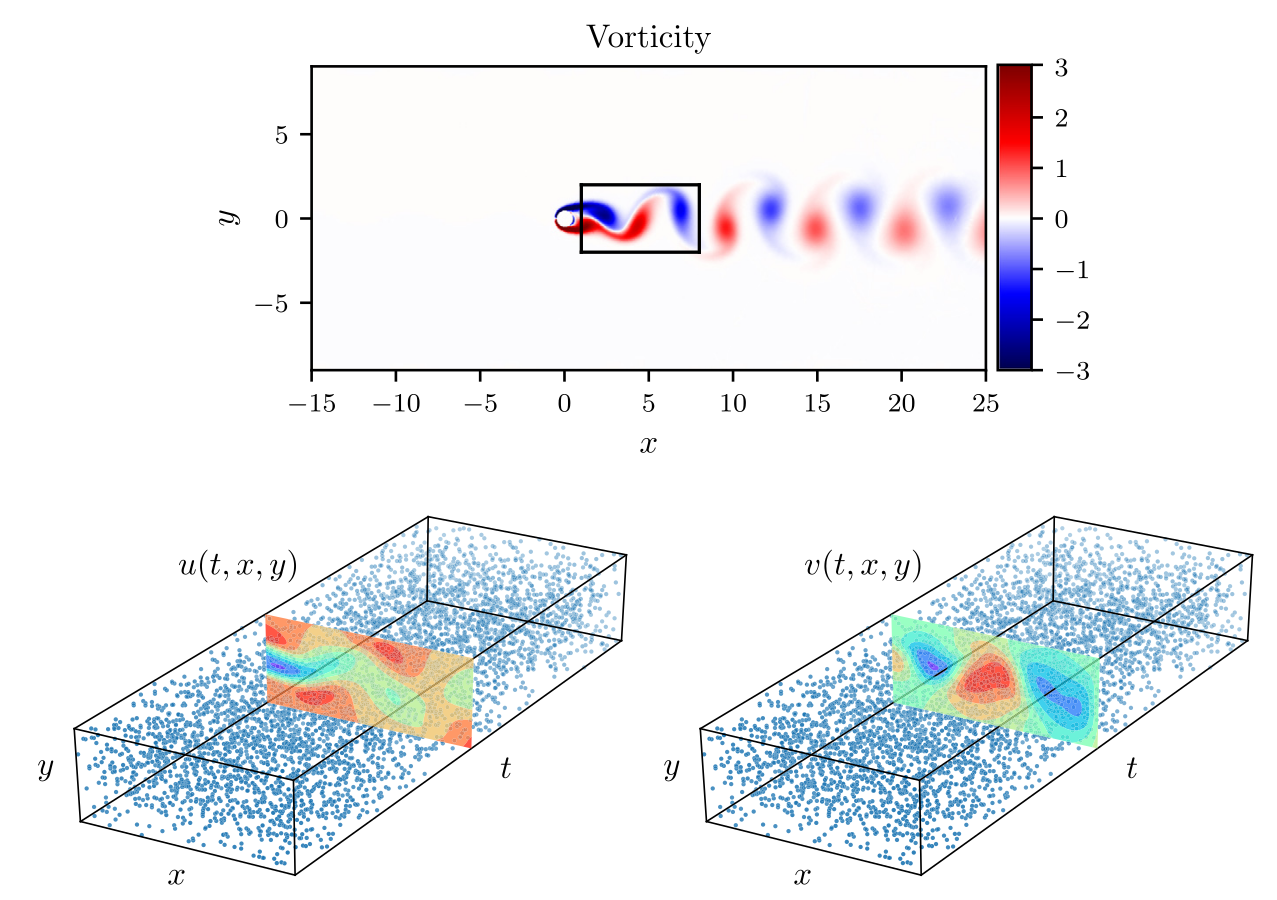
\includegraphics[width=0.8\textwidth]{img/navier-data.png}
\end{figure}
\end{frame}

\begin{frame}{Example: Navier-Stokes Equation}
\framesubtitle{Model}
The explicit form of the Navier-Stokes equations in two dimensions is:
\begin{align}
    u_t + \lambda_1(uu_x + vu_y) = -p_x + \lambda_2(u_{xx} + u_{yy})\\
    v_t + \lambda_1(uv_x + vv_y) = -p_y + \lambda_2(v_{xx} + v_{yy})
\end{align}
where:
\begin{itemize}
    \item $u(t, x, y)$ denotes the $x$-component of the velocity field.
    \item $v(t, x, y)$ denotes the $y$-component of the velocity field.
    \item $p(t, x, y)$ denotes the pressure.
\end{itemize}
Here, $\lambda = (\lambda_1, \lambda_2)$ are the unknown parameters.
\end{frame}

\begin{frame}
An extra equation for the conservation of mass of the fluid is included, 
\begin{align}
    u_x + v_y = 0
\end{align}
where is assumed that
\begin{align}
u = \psi_y \quad \text{and} \quad v = -\psi_x
\end{align}
for some latent function $\psi(t, x, y)$
\end{frame}

\begin{frame}{Example: Navier-Stokes Equation}
\framesubtitle{Architecture}
The neural network architecture is composed of:
\begin{itemize}
    \item input layer with 3 neurons $(t, x, y)$.
    \item 8 hidden layers with 20 neurons each.
    \item output layer with 2 neurons $(u, v)$.
\end{itemize}
\end{frame}

\begin{frame}{Example: Navier-Stokes Equation}
\framesubtitle{Results}
\begin{figure}[H]
    \centering
    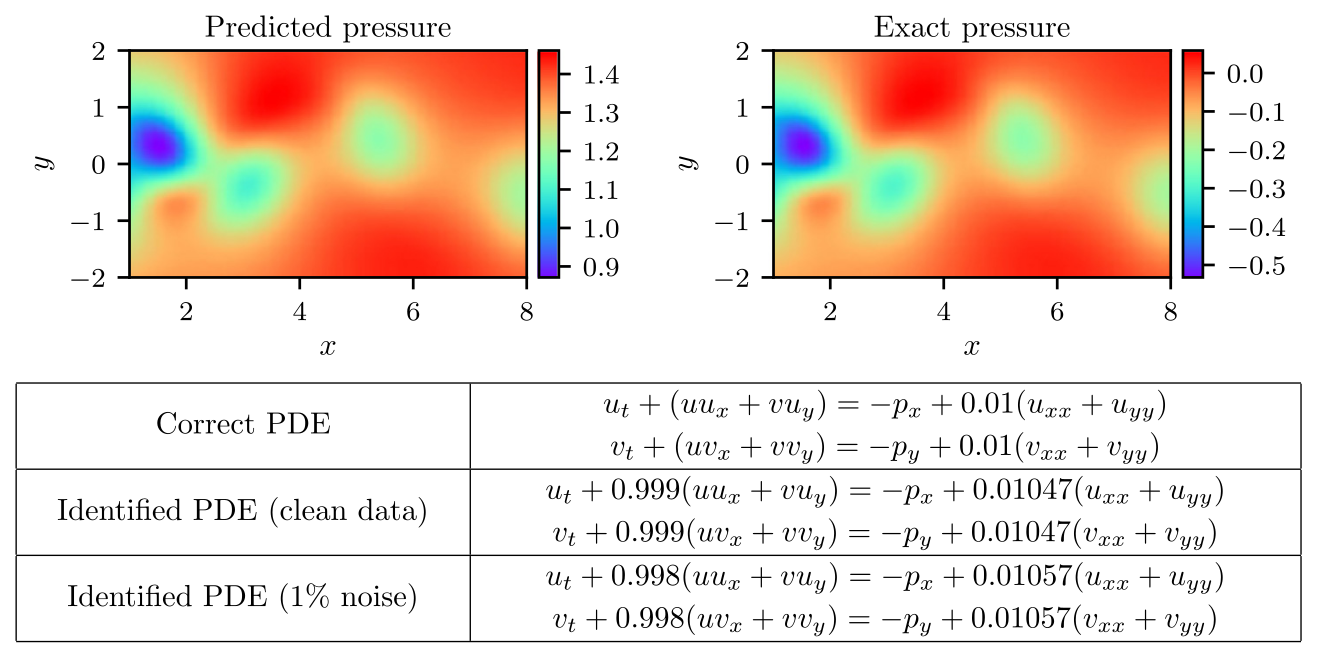
\includegraphics[width=0.8\textwidth]{img/navier-results.png}
\end{figure}
\end{frame}

\begin{frame}{Example: Navier-Stokes Equation}
\framesubtitle{Notes}
The example is fully available in the following repository:
\href{https://github.com/maziarraissi/PINNs}{maziarraisi/PINNs}.

To run the example, instantiate a conda environment with the following dependencies:

\texttt{conda create -n pinn-env python=3.8 tensorflow=1.15 numpy matplotlib scipy}

and activate the environment before running the code:

\texttt{conda activate pinn-env}

\end{frame}